\section{Tredje iteration}

\subsection{Integrationstest - Constant load}
\subsubsection{Udgang}
På figur~\ref{fig:realisering_udgang_e_filter_3} ses udgangen efter den er flyttet efter filtrene kondensatorerne danner. 
\begin{figure}[H]
	\center
	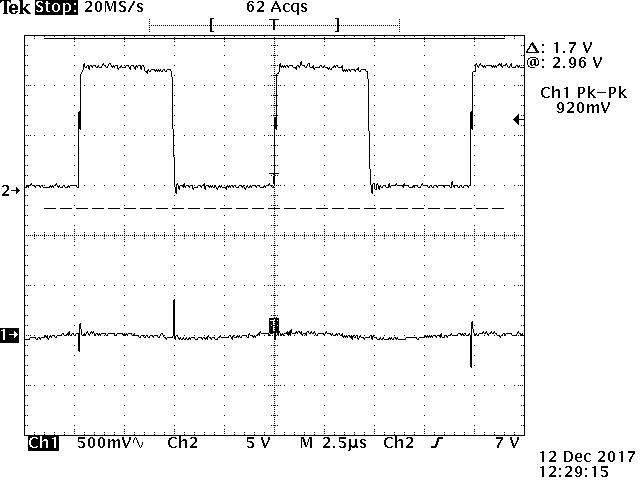
\includegraphics[max width=0.7\linewidth]{../dokumentation/tex/3iteration/billeder/Realisering/udgang_e_filter_3iteration.png}
	\caption{Udgangssignal efter filter - 3. iteration}
	\label{fig:realisering_udgang_e_filter_3}
\end{figure}
Switching spikes aflæses til at være ca. $920mV$ pk-pk.
Der er zoomet ind på udgangssignalet på figur~\ref{label}, hvor spændingsripplen kan aflæses til ca. $50mV$ pk-pk

\subsubsection{MOSFET}
Efter snubber kredsløbene er indsat, kan den nye realiserede drain spænding ses på figur~\ref{fig:realiseirng_snubber_MOSFET_3} 
\begin{figure}[H]
	\center
	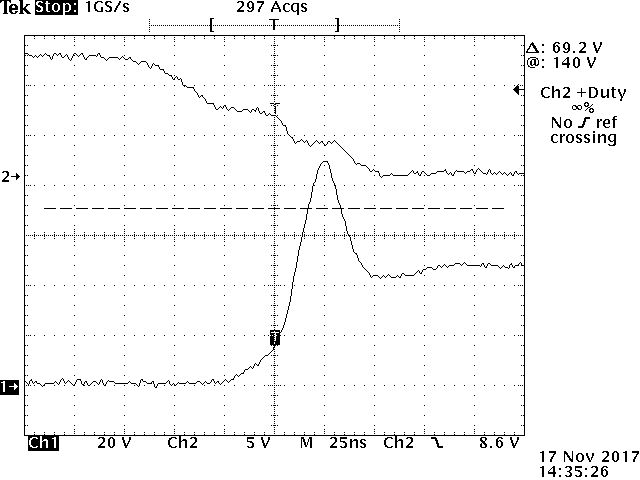
\includegraphics[max width=0.7\linewidth]{../dokumentation/tex/3iteration/billeder/Realisering/Realisering_switch_tid.PNG}
	\caption{Drain spænding efter snubber er tilføjet}
	\label{fig:realiseirng_snubber_MOSFET_3}
\end{figure} 
Der observeres ingen svingninger efter peaken.

\subsubsection{PWM-controller}
Tabel~\ref{tab:resultat_klkl} viser ændrede analyse-, simulerings- og realiseringsresultater. Det drejer sig om switch-tid og current sence filterets stigetid.
\begin{table}[H] 			
	\centering
	\begin{tabularx}{\textwidth}{|X|c|c|c|}
		\hline
		\textbf{Frekvens} & \multicolumn{3}{|c|}{\textbf{Resultat}} 		\\ \hline
		& A & S & R 									\\ \hline 
		$T_{ch}$ & $37.2ns$ & $29.4ns$ & $40ns$ 									\\ \hline
		$T_r$ & $100ns$ & $85ns$ & $100ns$					\\  \hline
	\end{tabularx}
	\caption{Resultater for analyse, simulering og realisering af switch-tid og current-sense filter stigetid}
	\label{tab:resultat_klkl}
\end{table}

\subsection{Tab}
Tabel~\ref{tab:realisering_tab_3} giver et overblik over sammenhængen imellem det analyserede, simulerede og realiserede tab for 3. iteration.
\begin{table}[H] 			
	\centering
	\begin{tabularx}{\textwidth}{|X|l|l|l|}
		\hline
		\textbf{\large Komponent} & \multicolumn{3}{|l|}{\textbf{\large Tab}} \\ \hline
		& A & S & R	\\ \hline
		\textbf{Transformator samlet} & $1.46\watt$ & $1.62\watt$ & $0.8W$ \\ \hline 
		Kernetab & $366m\watt$ & $311m\watt$ & \\ \hline
		Kobbertab & $1.09\watt$ & $1.31\watt$ & \\ \hline
		& &	& \\ \hline
		\textbf{MOSFET samlet} & $2.54\watt$ & $3.2\watt$ & $2.29W$ \\ \hline
		Conduction-tab & $1.06\watt$ &  &	\\ \hline
		Switch-tab & $1.48\watt$ & 	&		\\ \hline
		& &	& \\ \hline
		\textbf{Diode} & $1.13\watt$ & $1.47\watt$ & $1.77W$ \\ \hline
		& &	& \\ \hline
		\textbf{CS modstands tab} & $1.52\watt$ & $2.03\watt$ & \\ \hline
		& & &	\\ \hline
		\textbf{Snubber-kredsløb} & $220.9m\watt$ & $308m\watt$ & \\ \hline
		Primær snubber	& $132.5m\watt$	& $234m\watt$	&	\\ \hline
		Sekundær snubber &	$88.4m\watt$ &	$74m\watt$	&	\\ \hline
		& &	& \\ \hline
		\textbf{Total tab} & $6.87\watt$ & $8.63\watt$ & $5.9W$	\\ \hline
	\end{tabularx}
	\caption{Oversigt over analyseret, simuleret og realiseret tab}
	\label{tab:realisering_tab_3}
\end{table}

\subsection{Integrationstest - Gain-fase måling}
Med det ændrede kompenseringsnetværk bliver den realiserede gain-fase måling af det samlede system, som vist på figur~\ref{fig:Realisering_total_3}. Igen med det analyserede for at sammenligne.
\begin{figure}[H]
	\center
	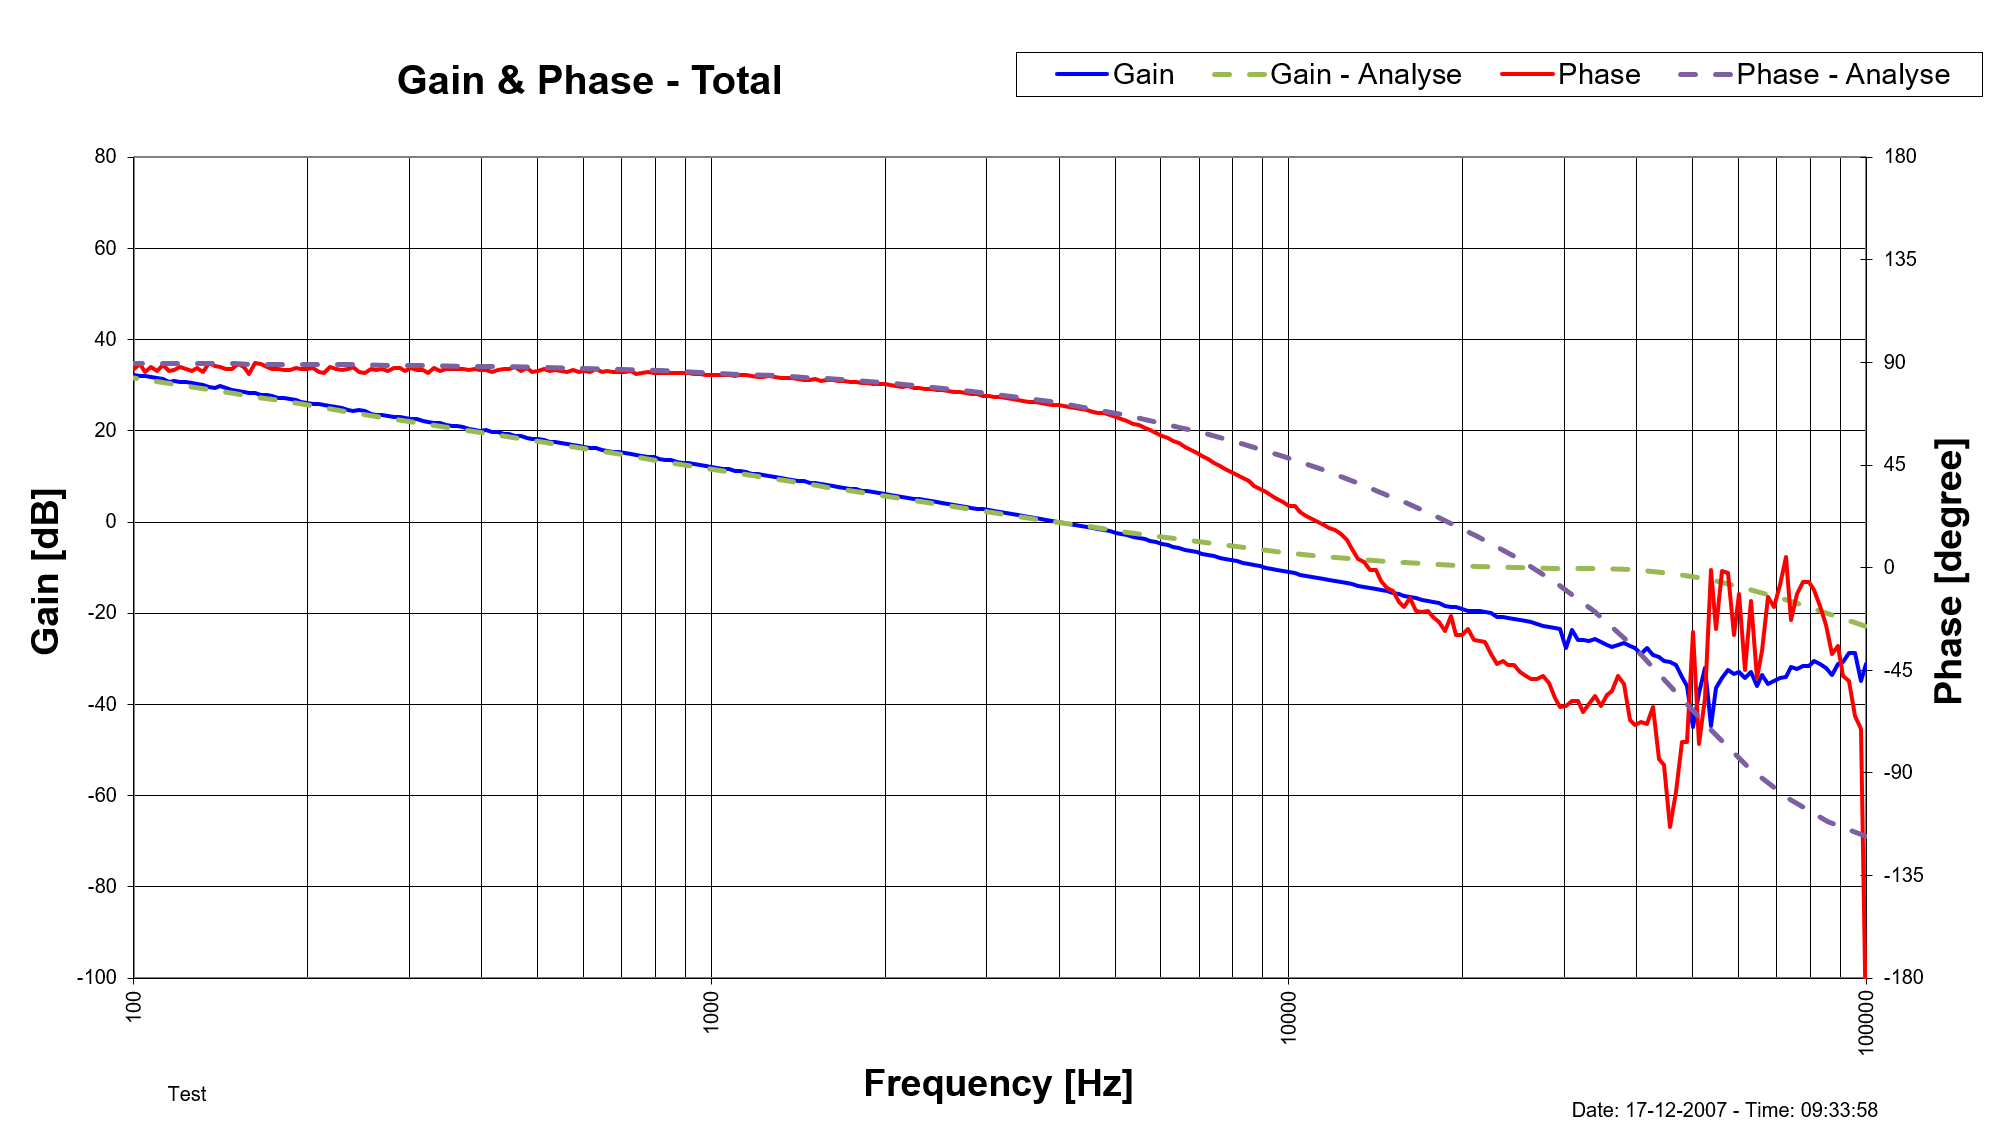
\includegraphics[max width=0.7\linewidth]{../dokumentation/tex/3iteration/billeder/Realisering/Realisering_gain_fase_total.PNG}
	\caption{Gain-fase måling af det samlede system}
	\label{fig:Realisering_total_3}
\end{figure}
Her aflæses den realiserede gain-margin til $14.5dB$. Fase-margin og båndbredde aflæses til hhv. $69.8^\circ$ og $3.86k\hertz$. Den analyserede gain-margin aflæses til $10dB$ med samme båndbredde og fase-margin som det realiserede.

\subsection{Load step}
På figur~\ref{fig:Loadstep3} ses det realiserede load step for 3. iteration.
\begin{figure}[H]
	\center
	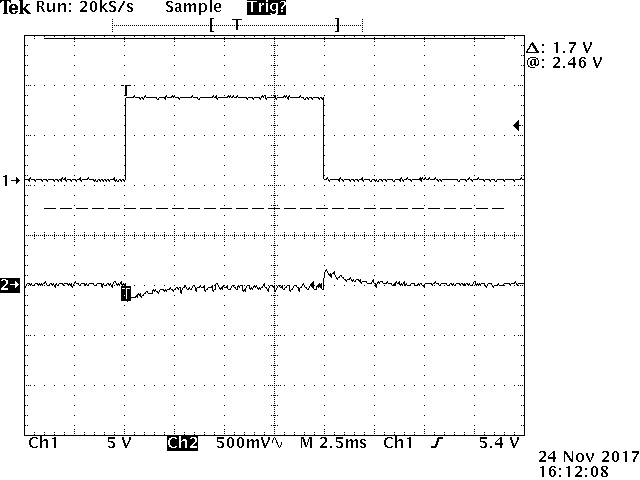
\includegraphics[max width=0.7\linewidth]{../dokumentation/tex/3iteration/billeder/realisering/Loadstep.PNG}
	\caption{Realiseret load step}
	\label{fig:Loadstep3}
\end{figure} 
Ved skiftet til $10\ohm$ falder spændingen med ca. $300mV$, og bruger $2ms$ på at regulere ind igen. Når loaden skifter tilbage til $20\ohm$ stiger spændingen med ca. $200mV$ og bruger $2ms$ på at regulere ind. 